\chapter{CellTAN: Cellular Time Activation Networks} \label{chap:chap4}

Distributed information systems characterized by time series data present various challenges, primarily due to their complex and dynamic nature. The sheer volume of data that must be processed and analyzed in real-time is a significant challenge, leading to concerns over storage, computation, and scalability. Moreover, data quality issues such as missing or incomplete data and data heterogeneity arising from sourcing data from disparate sources with varying consistency and structure further exacerbate these challenges. Another critical challenge of these systems is handling the temporal aspects of time series data, requiring specialized pre-processing, feature extraction, and modeling techniques. The distributed nature of these systems further complexifies matters, with issues encompassing data synchronization and accuracy being a common concern. Furthermore, their implementation in real-world applications requires robust mechanisms for data security and privacy, which adds a layer of complexity to the design and implementation of these systems.

\begin{figure}[h!]
    \centering
    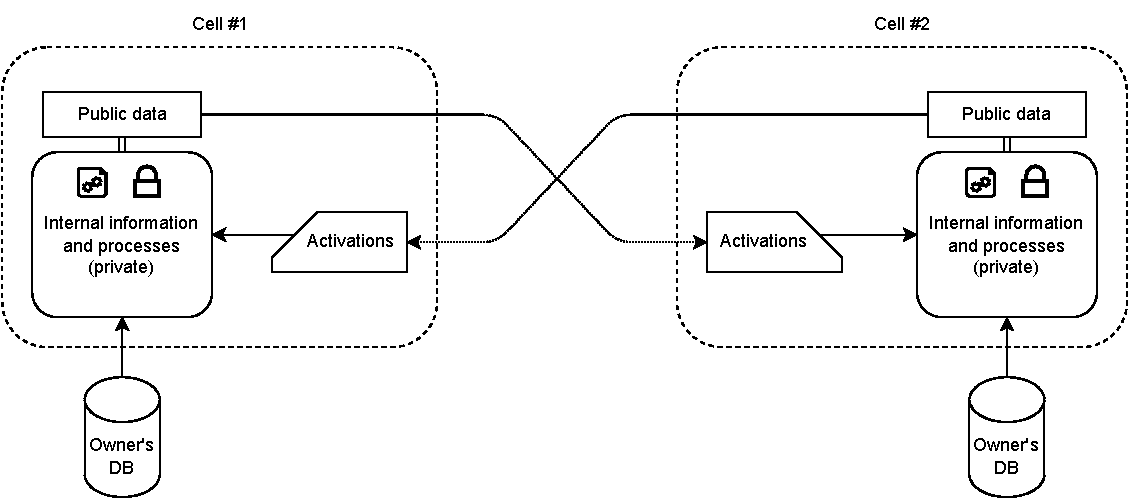
\includegraphics[width=12cm]{figures/chapter4/cell/intro.pdf}
    \caption{Simples CellTAN Network of two cells cooperating.}
    \label{fig:celltanintro}
\end{figure}

This chapter proposes a novel tool entitled CellTAN (Cellular Time Activation Network) that undertakes those challenges. CellTAN represents sparse yet interconnected components that function independently, cooperatively, and asynchronously. Inspired by other effective mechanisms like GNNs, CXNs, and Weighted Cross-Connection Networks (WCCNs), CellTAN uses a graph-like structure to represent a network of components with nodes and connections. Following the introductory chapters, its primary purpose is to detect abnormal scenarios on PV systems. However, its generalized formulation introduces other valuable features which come naturally from fulfilling this goal. Such are state estimation, forecasting, and capturing the value in data from different PV asset owners without violating their privacy. For briefness' sake, we will unfold details about its benefits during the rest of this chapter.

Instead of tackling fault detection and classification in a classical centralized manner, which is already extensively showcased throughout the literature, this tool approaches this problem with a paradigm change: a distributed and asynchronous data coherence system. By having a virtual representation closely related to the physical form of sparse systems, relationships between components can be leveraged to assess their correct (or incorrect) operation. While initially designed for photovoltaic (PV) systems, the concepts of cells, connections, neighbors, time series, and uncertainty are universal and applicable to other fields such as biology, physics, and more. Thus, the potential for generic applicability sparks the interest to not bake specifics of PV systems directly into this tool, allowing its usage for other subjects. Figure \ref{fig:celltanintro} represents minimal scenario for a network: only two cells. It showcases some terms specific to this tool, that might be difficult to grasp initially, such as trust, events, and activations. Consequently, the glossary in \ref{sec:glossary} and detailed explanations throughout this chapter serve to clarify them.

Vast and scattered information across multiple agents is a common scenario faced by the industry of AI for energy systems, which cannot be aggregated due to privacy and confidentiality reasons. Nevertheless, its conjunction could have a lot of added value, given the similarity of certain assets: PV plants (as well as wind farms) from different owners in neighboring geographical regions. This information-sharing potential for AI algorithms motivates the development of a mechanism that communicates information between differently owned assets without any of the compromises above. However, as stated before, data acquisition in PV scenarios is scarcely synchronous and might not occur in equal time resolutions for all the different components. The CellTAN addresses these issues with an instrument called \textbf{Time activations}. It proposes a new way of communication that decouples from the needs of units, sampling rate, and synchronization, avoiding resampling, normalization, or even obfuscation (to protect privacy). This mechanism is a core feature of the tool since it will be the means that will allow connecting different stakeholders' data, and section \ref{sec:thecell} develops this matter thoroughly. Likewise, succeeding sections formulate the working of the \textbf{Cell} and its interactions within the network. Since it is the core component, understanding its behavior is crucial for a complete understanding of the tool.

\section{Glossary} \label{sec:glossary}


\begin{itemize}
    \item \textbf{Knowledge base}: Refers to registered historical knowledge (samples) of time series variables.

    \item \textbf{Inputs}: Uniform fuzzy numbers (not necessarily, but it's the current choice) that represent one sample of the group of time series variables that define the state of a cell.

    \item \textbf{Outputs}: Similar to inputs, but obtained through some computations.

    \item \textbf{Time decay}: A process associated with increased uncertainty of variables over time.

    \item \textbf{Activations}: Timestamps of past occurrences on a knowledge base with a non-zero membership value against a set of recent inputs.

    \item \textbf{Events}: Occurrences that the cell reports back to the hub, usually triggered by exceeding parametrized thresholds.

    \item \textbf{Trust}: A decimal number that represents how coherent two cells' activations are with each other. Besides its instantaneous computed value, it can also come from a cumulative computation on a defined time window.

    \item \textbf{Hub}: The central component of the cell network, which facilitates its visualization, management, and expansion. It acts as the proxy agent between the cell's communication.

\end{itemize}

\section{The Cell} \label{sec:thecell}

% TODO falta mencionar que o dono da célula é que é responsável por estabelecer conexões

\subsection{Principles}

A cell is an independent entity composed of \textbf{data} and \textbf{processes}. The idea is to abstract fundamental system components (e.g. inverters, MPPT's) into this virtual entity. With an added intelligence layer and featuring a few different processes, it assesses its current state based on all available internal and external information, adding value to the existing data acquisition and monitoring systems. As an individual part of the system, it follows a set of rules that define its intrinsic and extrinsic behavior. These rules address data privacy, request boundaries, and real-world operational limitations.

\paragraph*{Independence} During operation, independence on neighbors or other network entities for continuous processing of outputs results in a more robust system and increases cell availability. Thus, given any connection cutoffs, the cell shall be unbothered by its surroundings and continue operating in an isolated state. Isolation is not preferred, but enduring it until outside contact is re-established avoids shutdown and startup procedures.

\paragraph*{Selfish Computations} The cell is selfish in that it will not perform any computations based on the request of others. This aspect creates a fundamental layer of protection against overloading the infrastructure in which it is deployed, which also increases availability.

\paragraph*{Data accessibility} Although selfish in computations, the cell shall provide access to select data valuable to the network. However, not all internal data is shared, and public data shall not compromise the cell's privacy (more on this later).

\subsection{Processes and Data}


The cell has a main process loop that executes a sequence of actions periodically: 

\begin{figure}[h!]
    \centering
    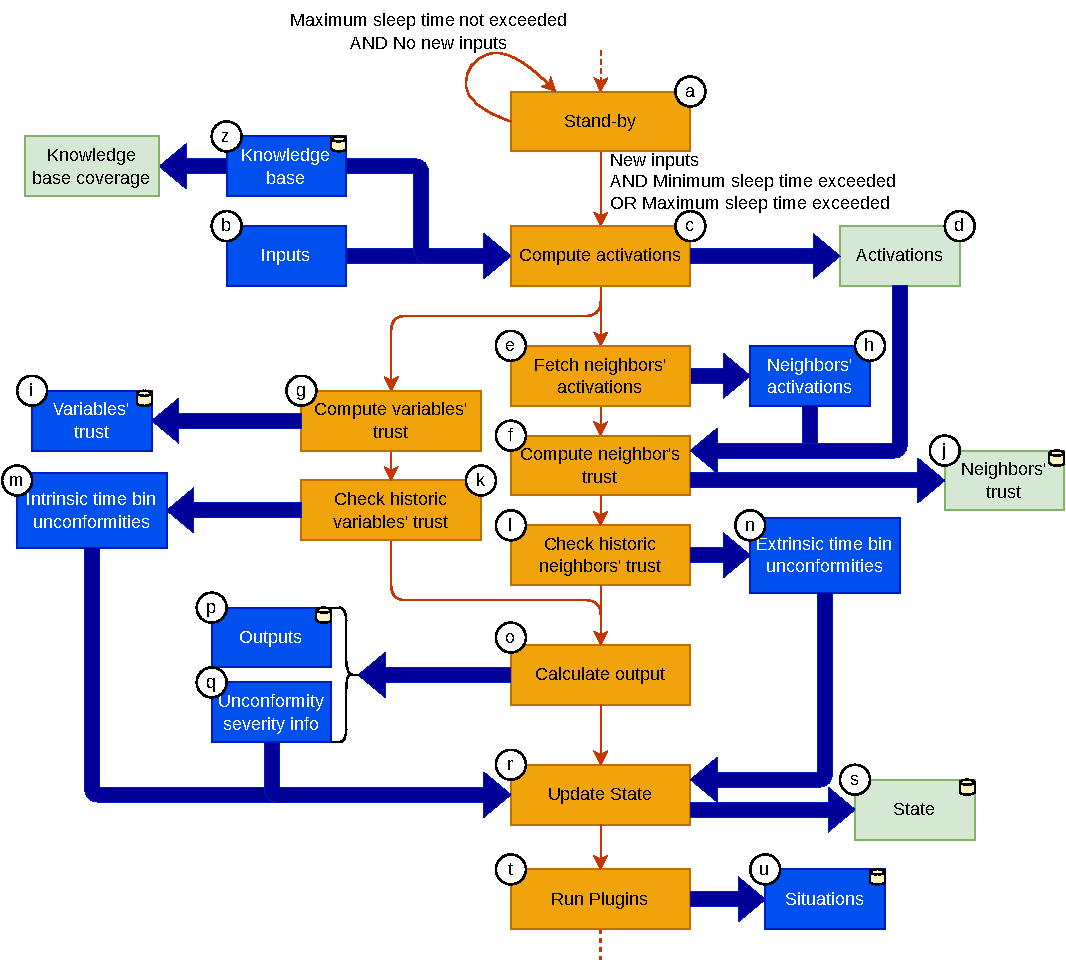
\includegraphics[width=12cm]{figures/chapter4/cell/processes.pdf}
    \caption{The cell's core sequence of processes (colored orange) and flow of data (colored blue).}
    \label{fig:cellprocesses}
\end{figure}

Figure \ref{fig:cellprocesses} showcases the cell's core procedures. It starts in a standby mode, which is only left when new information arrives or a predetermined amount of time has passed. This mode ensures that there isn't an unnecessary computational burden of repeating all other computations: they provide the most valuable results when new data is available. Nonetheless, defining a maximum sleep time ensures the cell's activations are periodically updated to reflect the neighbors' state and intrinsic uncertainty.

The process of computing activations relates to the temporal similarity extraction showcased in section \ref{subsec:tempsim}. It occurs twice because inputs only contain intrinsic information, while outputs aggregate intrinsic and extrinsic data (information from neighbors), and the latter is more worthy to the network. The cell makes this procedure's byproduct (Activations) publicly available, pictured in figure \ref{fig:celldata}.

Fetching neighbor's activations 

\begin{figure}[h!]
    \centering
    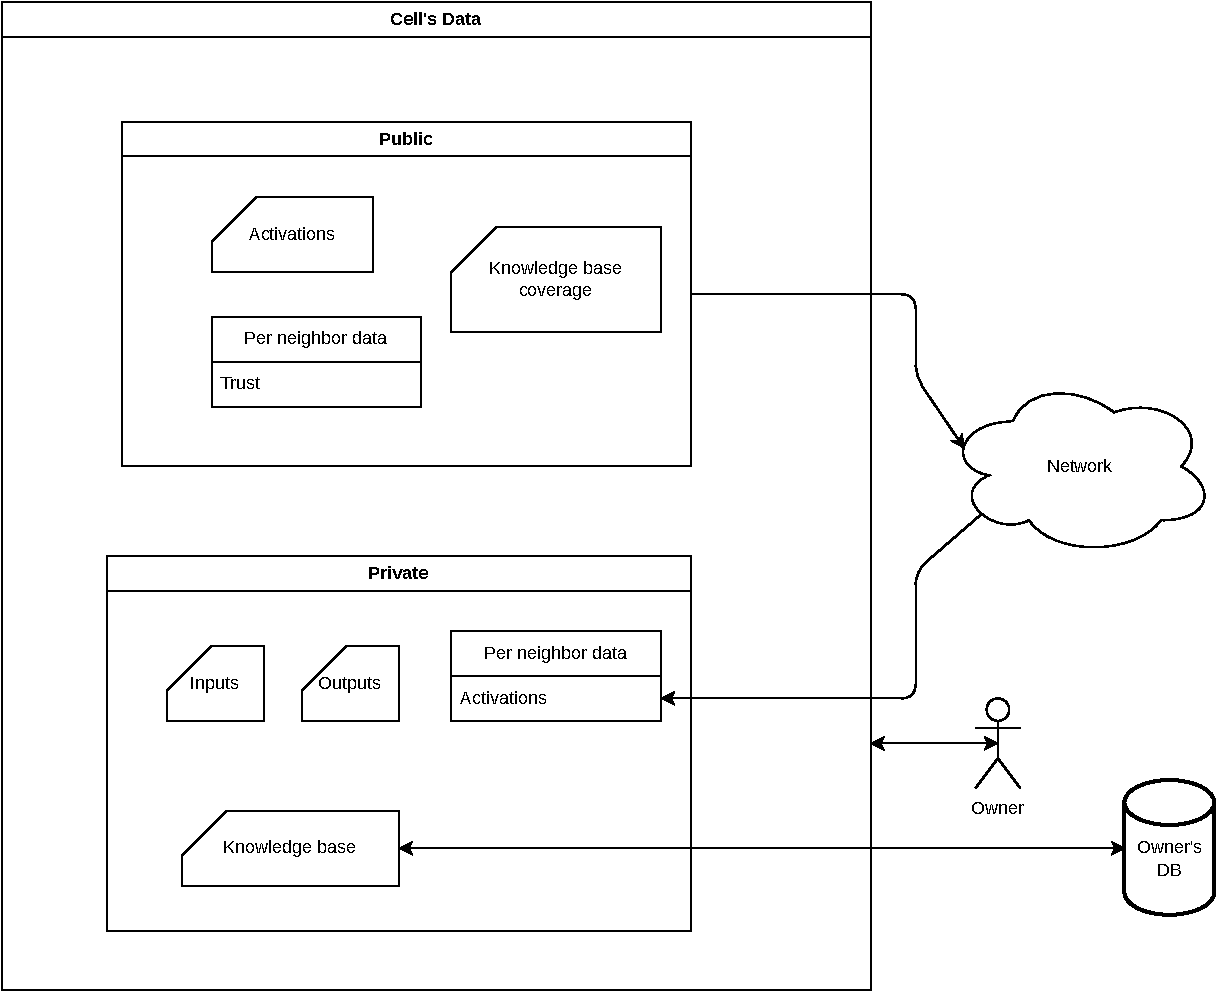
\includegraphics[width=\linewidth]{figures/chapter4/cell/data.pdf}
    \caption{The cell's public and private data attributes.}
    \label{fig:celldata}
\end{figure}

Figure \ref{fig:celldata} showcases the cell's public and private data attributes. The network may have access to its activations, knowledge base coverage, and neighbors' trust. Conversely, the cell extracts neighbors' activations from the network and gives its owner exclusive access to inputs, outputs, and knowledge base. The cell's knowledge base might only represent an interface with a private database (thus a bidirectional connection), not the data itself, since the owner might prefer a centralized storage server. The relationship between the owner and private cell data is bidirectional because it's his responsibility to update the inputs.


% TODO explicar processos da célula por alto

\subsection{Inputs and Outputs}

The cell has inputs and outputs. Both are a view of the values that define its variables at a given timestamp, which is continuously rolling. While inputs are directly associated with raw sampled data from the system (injected by the owner), outputs are a byproduct of internal processes. The latter should present more accurate information since it is based on internal and external data (ideally) and be helpful for the cell's owner to assess its state.

Representing the cell's variables in a fuzzy (or probabilistic) manner can better capture the inherent uncertainty in time series data. For the cell's inner workings, we chose that inputs and outputs are not represented by crisp values but rather by classical sets. However, they are not limited to this representation, with fuzzy numbers or probability distributions as alternatives. Besides, they can be subject to a process called \textbf{time decay}, which ensures that the passage of time negatively affects uncertainty (more on section \ref{subsec:timedecay}). This mechanism increases the robustness of the cell by acknowledging the value of time in assessing its current state.

Summing up, the following may characterize inputs and outputs:

\begin{itemize}
    \item Classical set: simple uncertainty band (e.g. uncertainty up, down, relative, etc);
    \item Fuzzy number: generalized fuzzy number representation \cite{Zhang2019} (e.g. triangular fuzzy number (a,b,d;h));
    \item Probability distribution: the distribution's characteristics (e.g. mean ($\mu$) and standard deviation ($\delta$) for Gaussian, the mean rate of occurrence ($\lambda$) for Poisson, etc.);
\end{itemize}

\begin{figure}[h!]
    \centering
    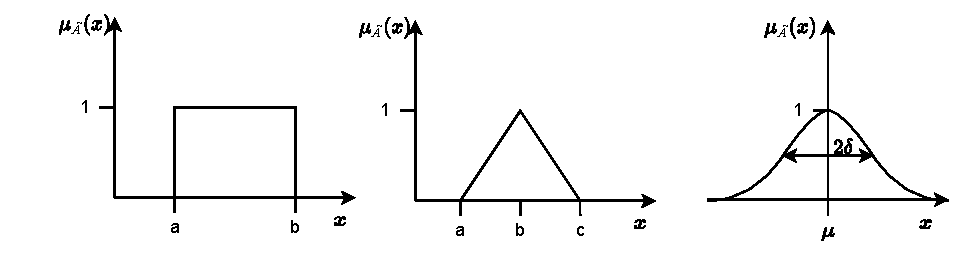
\includegraphics[width=15cm]{figures/chapter4/cell/classic_fuzzy_gaussian.pdf}
    \caption{Classical set, triangular fuzzy number, Gaussian distributions, and the associated membership function.}
    \label{fig:classicfuzzygaussian}
\end{figure}

Classical sets have pros and cons: many operations become more efficient, but we lose density information. Filtering historical data becomes trivial: a value lies within the bounds of the interval (membership value of one) or does not (membership value of zero). This more accessible representation will benefit some cell processes, primarily in temporal similarity extraction (\ref{subsec:tempsim}).

\subsection{Time decay} \label{subsec:timedecay}

In real-world dynamic systems that involve data acquisition, the certainty of the data collected tends to fade over time due to the nature of the data acquisition process. Typically, the most recent data is the most accurate representation of the system's current state, and as time elapses, the accuracy of previous data points decreases. This occurs naturally due to various factors such as environmental changes, equipment degradation, or other system's dynamics. As a result, it is crucial to consider the time dimension when analyzing dynamic systems and to develop methods that can account for the decay in data certainty over time.

As stated before, and towards considering the time dimension for the current state of a cell, we formulate a \textbf{time decay} method to ensure a more truthful and reliable assessment of the cell's current state. During the standby stage, this process ensures that the inputs and outputs suffer an increase in uncertainty, which is has different side effects depending on what represents them (classical set, fuzzy number or probability distribution).

Consider the following example of converting a crisp value and uncertainty to a classical set:

$$x = 5 \pm 1 \rightarrow [5-1, 5+1] = [4, 6]$$

To simulate the increase in uncertainty over time, we can apply the following formula to each bound:

\begin{equation}
lower = lower - (lower - minimum) \times \frac{age}{decay}
\end{equation}

\begin{equation}
upper = upper + (maximum - upper) \times \frac{age}{decay}
\end{equation}

The $age$ variable refers to the time difference between the present time and the instant of data acquisition. For implementation, the time unit considered is the second. The $decay$ is a parametrized constant (same unit as $age$) that defines the time it takes for the set to expand into its limits when starting from the median. It is chosen based on the characteristics of the variable, i.e., knowledge of its uncertainty over time. However, a good starting point is defining it as equal to the data acquisition period so that the set expands entirely until a new value is acquired.

\begin{figure}[h!]
    \centering
    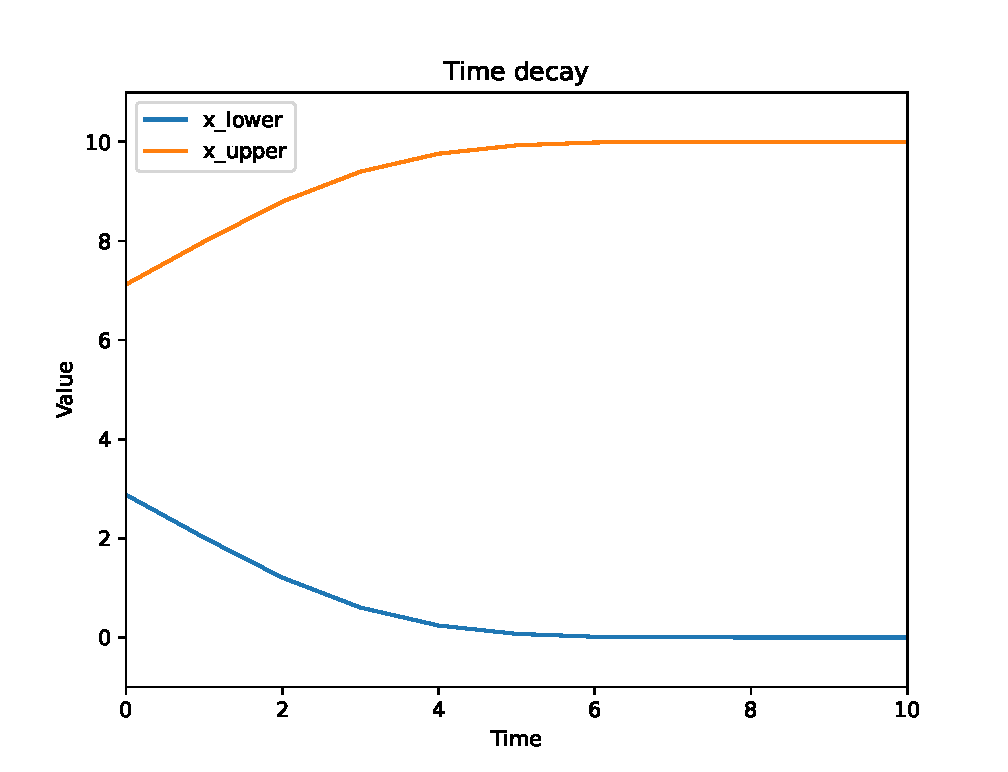
\includegraphics[width=10cm]{figures/chapter4/cell/time_decay.pdf}
    \caption{Visualization of the effect of time decay on $x_{lower}$ and $x_{upper}$.}
    \label{fig:timedecay}
\end{figure}

Table \ref{tab:timedecay} and figure \ref{fig:timedecay} represent the expansion of the set throughout a period equal to the decay parameter (ten seconds). When $x$ reaches the age of ten seconds, its set represents complete uncertainty since its bounds become similar to the variable limits ($x_{min}$ and $x_{max}$). We can see that the decreasing difference between the bounds and maximum/minimum values causes attenuation in the decay curve, as it displays a non-linear behavior. This behavior seems appropriate according to the reality of systems: as a variable becomes more uncertain, there is less potential for its uncertainty to increase.


\subsection{Temporal similarity extraction} \label{subsec:tempsim}

Temporal similarity extraction is the process of identifying recurring patterns in time series data. It involves the identification of past instances where the current state is observed to extract useful information about the system's behavior over time. By identifying historical periods with similar conditions, temporal similarity extraction can help assess the current state or predict future trends. This technique is common in statistics for purposes such as estimation and forecasting.

Using sets or probability distributions to filter historical data is one approach to simplify the process of temporal similarity extraction in multivariate time series data while also making it more robust against noisy or incomplete data. This approach assigns membership values to each data point in the time series based on the corresponding set (or distribution) generated from the current cell inputs. By eliminating samples past a certain threshold, we can form the outputs. The possibility of this process is one of the reasons for deciding to represent the inputs and outputs of the cell in a fuzzy manner. 

The proposal for similarity extraction in the cell consists of receiving new values (inputs) for the cell's variables from a data source (sensors or other data acquisition equipment, calculations, forecasting, etc.), generating a classical set, fuzzy number, or probability distribution from them, and then applying the bounds/membership function or probability density function to the knowledge base (see figure \ref{fig:solo_state_estimation}). When historical samples are associated with membership values, there may be a process for determining outputs by combining data and membership values.

The initial choice is to use classical sets since filtering history becomes trivial and efficient: restrict the knowledge base to samples where all variables belong to the corresponding interval. Generating outputs with these can be as simple as constructing new sets based on the bounds of filtered knowledge (samples with membership equal to one). When filtering historical data with two or more variables, there is a trend of narrowing down the resulting data's space due to the intersection of constraints. Therefore, this process should result in sets that are an equal or better assessment of the present state (than the sets generated by inputs). However, filtering might also result in zero samples (membership value of zero on all knowledge base's rows), which indicates not having "memory" of any similar occurrence. This zero-sample filter is an excellent indicator for potentially anomalous scenarios, primarily if we know that the knowledge base is statistically representative of the variables in the cell.

This process also makes possible for simple forecasting. Considering an offset (arbitrary number of rows forward) in the activations, the temporal similarity extraction and computation of outputs results in future values. So, cells may either compute outputs related to the present or future. Nonetheless, this temporal shift might be difficult to achieve if data samples arrive at randomly spaced intervals of time, thus would only be straightforward for systems with time-consistent data acquisition.

The following examples consider that $t=0$ is associated with the present, and $\mu$ represents membership functions.

\paragraph{Self-similarity}
Having a knowledge base and input variables, the cell can perform intrinsic temporal similarity extraction.
Consider the a cell that is characterized by two variables, which are a function of time: $x(t)$ and $y(t)$.
Assume that, at a given instant, these are the new cell inputs:

\begin{equation}
    x(0) = 1.0 \rightarrow \mu_{x(0)}(x) =
    \begin{cases}
        1, & x \in [0.9, 1.1]    \\
        0, & x \notin [0.9, 1.1] \\
    \end{cases}
\end{equation}

\begin{equation}
    y(0) = 2.0 \rightarrow \mu_{y(0)}(y) =
    \begin{cases}
        1, & y \in [1.8, 2.2]    \\
        0, & y \notin [1.8, 2.2] \\
    \end{cases}
\end{equation}

The membership functions $\mu$ are generated considering that $x$ and $y$ are characterized by uniform and symmetrical uncertainty and that the received samples of $x(0)$ and $y(0)$ represent their median.

\begin{figure}[h!]
    \centering
    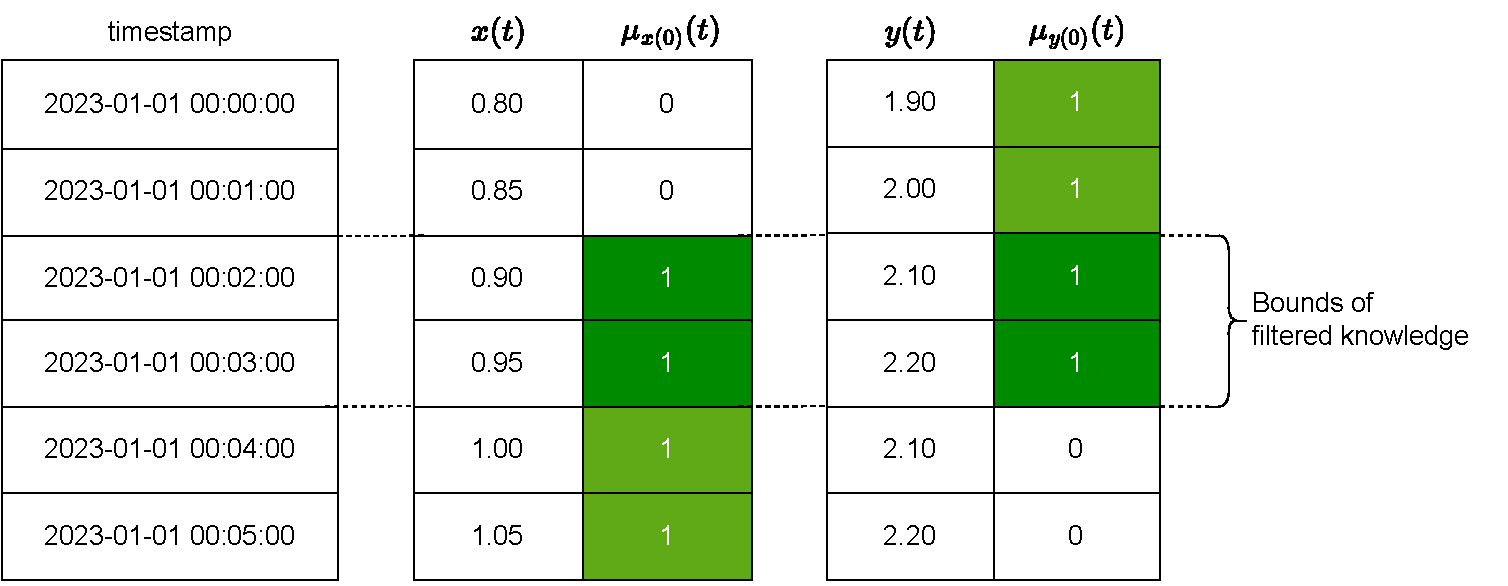
\includegraphics[width=\linewidth]{figures/chapter4/cell/solo_state_estimation.pdf}
    \caption{Visualization of a self-similarity extraction example.}
    \label{fig:solo_state_estimation}
\end{figure}


With the knowledge base represented in figure \ref{fig:solo_state_estimation}, the resulting activations will be 2023-01-01 00:02:00 and 2023-01-01 00:03:00. These are the timestamps of past instances where the cell's variables have values belonging to the set generated from new inputs. Now we can also infer that the actual values of $x$ and $y$ should reside in a set constrained by the filtered historical data ($x(t)$ and $y(t)$). Therefore, the outputs based on self-similarity extraction are:

\begin{equation}
    x'(0) \in [0.90, 0.95]
\end{equation}

\begin{equation}
    y'(0) \in [1.80, 2.20]
\end{equation}

These results confirm that we achieve outputs with less uncertainty only depending on intrinsic processes and private data.

\paragraph{Mutual Similarity}

Extending similarity extraction to multiple cells is a relatively trivial process. Suppose a cell has access to another's activations at the same rolling timestamp and for a historical window that intersects its knowledge base. In that case, it can use that information to refine the intrinsic temporal similarity extraction result. Using sets, this can occur by joining intrinsic and extrinsic membership values by aggregation (e.g. sum, multiplication, average, etc).
Although simple, this process has some tricky requirements, such as not allowing a time difference between the computation of membership values of different cells to avoid joining incoherent information, and 
% Capacidade de estimação de estado intrínsica + extrínsica

\subsection{Connections and Trust}

Connections are the essence of forming the CellTAN network. Mutual similarity extraction and comparison of activations can only occur in cell neighborhoods. These links may have associated indicators that describe the cells' relationships, and a critical metric we consider for anomaly detection is entitled \textbf{Trust}.

Each cell has a unique identifier, generated upon creation and independent of the name attributed by the owner. This ID serves to register cells and better manage the network. Since interconnections require an agent to keep track of these IDs and correctly direct traffic, we introduce a component entitles \textbf{Hub} for keeping track of registered cells in the network and their corresponding id's. By having a central component which provides global network visibility, connections are easier to form.


\subsubsection{Trust computation}


% TODO só fazer depois de confirmar as equações com o prof
\dots


\subsection{Events}

\dots


\section{The Hub}

The CellTAN tool is supposed to be easily accessible for different assets and owners in any given location. However, for privacy and security reasons, monitoring equipment and other smart devices (IoT, servers, etc.) in PV plants and the owner's database are usually protected from unwanted outside connections. Because of this, the CellTAN network owner can act as a proxy and be responsible for arranging the necessary connections between the equipment of different asset owners and the network. This way, all traffic is routed through its system, which solves the issues mentioned before but possibly introduces a bottleneck and affects availability. These downsides are inevitable for aggregating distributed systems and sharing information between otherwise reserved agents. Besides being a proxy, other responsibilities associated with the Hub are:

\begin{itemize}
    \item Provide network visibility: cells and connections;
    \item Receive events from cells;
    \item Cell connection proposal.
\end{itemize}

Adding this component permits visualizing all the cells registered in the system and their public data. This 

\section{Implementation}

\subsection{Programming and Infraestructure}

Materializing both the Cell and the Hub happened through Python modules. It was developed using a mix of the OOP (Object Oriented Programming) and FP (functional programming) paradigms and features a structure familiar with the descriptions in previous sections. Using Python for the implementation of the CellTAN comes with the following advantages:

\begin{itemize}
    \item Easy to read and write code, requiring less syntax for complex operations compared to low-level languages;
    \item Extensive availability of libraries and tools;
    \item Deployment ease: doesn't have to compile, only needing an interpreter and dependencies to run;
    \item Big community support, with many resources publicly available online (e.g. documentation, tutorials, etc.). 
\end{itemize}

% imagem com as tecnologias em anexos talvez

Docker containers \cite{docker} are the infrastructure choice for deploying cells and the Hub. They allow running software as containerized applications, with all the necessary dependencies installed virtually. It acts as a separate system built for running the application instead of relying on the host's OS (Operating System) and running bare-metal. This execution strategy adds an isolation layer between the program and the host machine, increasing safety and making the "production" environment more predictable and stable. An overview of the technology stack utilized and proposed for the software products created in this work is pictured in appendix \ref{ap1:techstack}.

% dockerfile em anexos?

\subsection{Cell configuration and deployment}


Configuring cells can be done through configuration files (one per cell). They should contain the cell variables' definitions, database credentials, hub credentials, and all other parameters. Because of its simplicity, we chose the YAML serialization specification \cite{yaml} to parse these configurations. A walkthrough of the cell configuration and expected file structure is present in appendix \ref{ap1:config}


% meter anexo para explicação das configs com screenshot de configuração exemplo
